%%%%%%%%%%%%%%%%%%%%%%%%%%%%%%%%%%%%%%%%%%%%%%%%%%%%%%
% Esse template foi um fork do 
% https://github.com/lucasmsoares96/Template-Monografia-CEFET-MG
% Modificado para atender aos padrões da FACE-UFMG
% Já está usando as atualizações da abnt de 2023 para as citações
% Esse documento é dividido em três arquivos tex diferentes: pre_textual.tex, textual.tex e pos_textual.tex
%
% Pedro Benner
%%%%%%%%%%%%%%%%%%%%%%%%%%%%%%%%%%%%%%%%%%%%%%%%%%%%%%

\documentclass[a4paper,12pt,oneside]{memoir}
\usepackage{FACE}

\addbibresource{bibliografia.bib}


% Configurações do Documento
\title{Título do Trabalho:}
\subtitle{subtítulo do trabalho (se houver)}
\author{Nome do Autora}  

\date{2024}
\location{Belo Horizonte}

\advisor{Orientador: Título Nome}
\coadvisor{}

\committeeone{Nome do Orientador\\ Titulação}
\committeetwo{Nome do Avaliador\\ Titulação}
% \committeethree{Título Nome\\ Titulação} Se houver terceiro membro da banca modificar também o arquivo FACE.sty


% Lembre de colocar a data real no lugar de "\today" antes de imprimir a folha de aprovação
\committeedate{\today}

\institution{
  Universidade Federal de Minas Gerais
  \\
  Faculdade de Ciências Econômicas
  \\
  Departamento de Ciências Econômicas
}

\preamble{Monografia apresentada ao Departamento de Ciências Econômicas da Universidade Federal de Minas Gerais, como requisito parcial à obtenção do título de Bacharel em Ciências Econômicas.}


\usepackage{lipsum}    % gera texto aleatório (remover)

\begin{document}

\frontmatter
\pretextual

\maketitle
\makecover % folha de rosto               (obrigatório)
% Se houver errata, deverá ser incluída após a folha de rosto


% ---
% Após a apresentação do trabalho incluir o pdf com a folha com as assinaturas utilizando os seguintes comandos.
% 
% \begin{titlingpage*}
% \includepdf{folha_assinada.pdf}
% \end{titlingpage*}
%
\makeapproval %  (obrigatório)

\dedication{Folha na qual o autor presta uma homenagem ou dedica seu trabalho. Não leva título e a dedicatória deve aparecer na parte inferior da página, a 8cm da margem esquerda.}

\clearpage\pagestyle{empty}
\chapter*{Agradecimentos}
"Expressos pelo autor que presta seu reconhecimento às pessoas e instituições que
colaboraram na elaboração do seu trabalho. Não leva indicativo numérico e o título
deve ser centralizado na folha, utilizando a mesma tipologia das seções primárias do
texto." conforme o manual de normalização página 10.
\clearpage

% \epigraph{O ontem é história, o amanhã é um mistério, mas o hoje é uma dádiva. É por isso que se chama presente.}{Mestre Oogway}%       (opcional)

\epigraph{only a boring man will always want things to match;
real quality lies in irregularity}{Yoshida Kenkō}

\clearpage\pagestyle{empty}
% \begin{abstract}
    O resumo deve ressaltar o objetivo, o método, os resultados e as conclusões do documento. A ordem e a extensão destes itens dependem do tipo de resumo (informativo ou indicativo) e do tratamento que cada item recebe no documento original. Deve ser precedido da referência do documento, com exceção do resumo inserido no próprio documento, e ser composto de uma sequência de frases concisas, de cunho afirmativo e sem enumeração de tópicos, dado que se recomenda o uso de parágrafo único. As palavras-chave devem figurar logo abaixo do resumo, antecedidas da expressão palavras-chave, e finalizadas também por ponto.
    É importante evitar:
    \begin{enumerate}
        \item símbolos e contrações que não sejam de uso corrente;
        \item fórmulas, equações, diagramas e similares que não sejam absolutamente necessários; quando seu emprego for  imprescindível, deve-se defini-los na primeira vez em que aparecerem.
    \end{enumerate}
    Quanto à extensão, os resumos devem ter:
    \begin{enumerate}
        \item de 150 a 500 palavras os de trabalhos acadêmicos (teses, dissertações e outros) e relatórios técnico-científicos;
        \item de 100 a 250 palavras os de artigos de periódicos;
        \item de 50 a 100 palavras os destinados a indicações breves.
    \end{enumerate}
    Como tratado, o resumo deve ser seguido das palavras representativas do conteúdo do trabalho, isto é, palavras-chave, ou descritores, no idioma em que foi redigido (mínimo 3). Elas devem ser separadas por ponto e virgula e finalizadas com ponto final.
    \\ \\
    \textbf{Palavras-chave:} Palavra-chave 1; Palavra-chave 2; Palavra-chave 3; Palavra-chave 4; Palavra-chave 5.
\end{abstract} %        (obrigatório)

\begin{abstract}
    É a apresentação concisa dos pontos relevantes do texto, fornecendo uma visão rápida
    e clara do conteúdo do trabalho e das conclusões alcançadas, de tal forma que este
    possa dispensar a consulta ao original. Deve ter uma extensão de 150 a 500 palavras.
    Abaixo do resumo devem figurar as palavras-chave, representativas do conteúdo do
    trabalho. Devem ser precedidas da expressão Palavras-chave: separadas entre si por
    ponto e finalizadas também por ponto.
    \\ \\
    \textbf{Palavras-chave:} Palavra-chave 1; Palavra-chave 2; Palavra-chave 3; Palavra-chave 4; Palavra-chave 5.
\end{abstract}
\clearpage

% \begin{otherlanguage}{english}
    \begin{abstract}
        Tradução do resumo em português.
        \\ \\
        \textbf{Keywords:} Keywords 1; Keywords 2; Keywords 3; Keywords 4; Keywords 5.
    \end{abstract}
\end{otherlanguage} % 
\begin{otherlanguage}{english}
    \begin{abstract}
        Tradução do resumo em língua vernácula preferencialmente para o inglês. Deve ser
        seguido das palavras-chave traduzidas para a mesma língua.
        Localizado logo após o resumo em língua vernácula.
        \\ \\
        \textbf{Keywords:} Keywords 1; Keywords 2; Keywords 3; Keywords 4; Keywords 5.
    \end{abstract}
\end{otherlanguage}
\clearpage


\listoffigures* %                          (opcional)
% \listoftables*  %                          (opcional)


% --- Lista de abreviaturas (opcional)
% Lista de abreviaturas usando o pacote acronym. As abreviaturas precisam ser usadas no texto usando o comando \ac{} na primeira vez que for invocado ele substituirá a descrição longa e nas vezes subsequentes incluirá apenas a sigla com um link para a definição na lista de abreviaturas 
% ---

% \chapter*{Lista de Abreviaturas e Siglas}
% \begin{acronym}
%     \acro{API}{Interface de Programação de Aplicativos, do inglês \textit{Application Programming Interface}}
%     \acro{CPU}{Unidade Central de Processamento, do inglês \textit{Central Processing Unit}}
%     \acro{DAG}{Grafos Acíclicos Dirigidos, do inglês \textit{Directed Acyclic Graph}}
%     \acro{GC}{Coletor de Lixo, do inglês \textit{Garbage Collector}}
%     \acro{VM}{Maquina Virtual, do inglês \textit{Virtual Machine}}
% \end{acronym}


% ---
% inserir lista de símbolos
% ---
\nomenclature{$\alpha$}{Letra grega minúscula alpha}
\nomenclature{$\rightarrow$}{"Tem seu valor alterado para..."}
\nomenclature{$\propto$}{"é proporcional à..."}
\nomenclature{$\lesssim$}{"Aproximadamente menor que..."}
\nomenclature{$\gg$}{"Muito maior que..."}
\printnomenclature

\clearpage

\tableofcontents* %                        (obrigatório)

\mainmatter
\textual
\chapterstyle{texto}

% ----------------------------------------------------------
% Introdução (exemplo de capítulo sem numeração, mas presente no Sumário)
% ----------------------------------------------------------
\chapter{Introdução} \label{intro}
% ----------------------------------------------------------

\lipsum[2]


\chapter{Revisão Bibliográfica} \label{revisao}

Primeiro, é preciso preencher o arquivo Dados.tex para que suas informações sejam, devidamente passadas em todos os campos necessários no documento. Se sua banca tiver um terceiro avaliador favor alterar o arquivo em Pacotes/Face.sty e a linha em Dados.tex.

A seguir mostro os comandos principais a serem utilizados. Primeiramente, aqui está a citação com autor no final da frase \cite{nome_facil}. E também uma citação segundo \textcite{nome_facil} que aparece no meio da frase. Além disso é sempre possível também incluir uma citação longa que aparece com recuo conforme:

\begin{quote}
    \lipsum[3]\cite{nome_facil}
\end{quote}

Novos capítulos podem ser criados usando o comando \verb!\chapter!. Cada capítulo pode ser referenciado dinamicamente pelo \verb!\label! que acompanha ele. Assim se na frente a ordem do capítulo mudar a referencia se altera automaticamente no texto como vimos no capítulo \ref{revisao}. Novas seções podem ser iniciadas através do comando \verb!\section! . E também temos subsections e subsubsections de formas análogas.

Figuras podem ser inseridas no overleaf de maneira simples utilizando a interface gráfica. Aqui está uma figura num jeito mais ou menos pronto caso queira copiar. A figura também tem uma label que pode ser referenciada como na Figura \ref{fig:lei_potencias}. As figuras no latex são floats e possuem esses parâmetros h,b,t,p que influenciam seu posicionamento e dá pra saber mais \href{https://tex.stackexchange.com/questions/39017/how-to-influence-the-position-of-float-environments-like-figure-and-table-in-lat}{Nesse linkizinho do stackexchange de tex}. Que inclusive vai ser seu melhor amigo quando surgirem os primeiros problemas. 

\begin{figure}[h]
    \centering
    \caption{Simulação de uma lei de potência}
    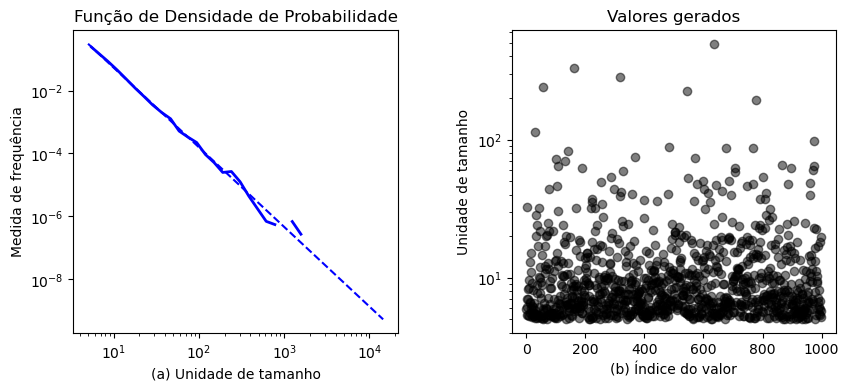
\includegraphics[width=1\linewidth]{Imagens/duas.png}
    \label{fig:lei_potencias}
    \captionsetup{font=footnotesize}
    \vspace*{-7mm}
    \caption*{Fonte: Elaboração Própria}
\end{figure}


Também temos equações alinhadas pra ficarem bem bonitinhas. Com novas labels pra gente referenciar. Como nas equações \eqref{matrix_minus}, \eqref{matrix_x} e \eqref{matrix_y}. E se quiser botar uma matemática na linha mesmo basta Digitar entre simbolozinhos de dólar $x=y-x$

\begin{align} 
M(x,y) & \rightarrow  M(x,y) - 4 \label{matrix_minus}\\ 
M(x\pm 1,y) &\rightarrow  M(x\pm 1,y) + 1 \label{matrix_x}\\
M(x,y \pm 1) &\rightarrow  M(x, y\pm 1) + 1 \label{matrix_y}
\end{align}

Por fim um outro comando fácil de mostrar é o de notas de rodapé. \footnote{Que colocam uma notinha de rodapé lá embaixo na página}

\chapter{Modelagem} \label{modelagem}

\lipsum[5]
\section{Descrição do Modelo} \label{descrição}

\lipsum[5]

\section{Desenvolvimento do Modelo} \label{desenv}

\lipsum[10]

\subsection{Exploração do modelo}

\lipsum[10]

% ---
% Conclusão
% ---
\chapter{Conclusão} \label{conclusao}

\lipsum[10]

% Conserta o indent para alinhar conforme padrão de normalização
\addtocontents{toc}{\cftsetindents{chapter}{1.5cm}{3em}}
\addtocontents{toc}{\cftsetindents{section}{0cm}{1.5cm}}
\addtocontents{toc}{\cftsetindents{subsection}{0cm}{1.5cm}}
\addtocontents{toc}{\cftsetindents{subsubsection}{0cm}{1.5cm}}
\addtocontents{toc}{\protect\renewcommand{\protect\cftchapteraftersnum}{\enskip\textemdash\enskip}}


\printbibliography[title={REFERÊNCIAS}, heading=bibintoc] %

% ---
% Inicia os apêndices
% Para as seções nos apêndices usar o comando \section* que não adiciona a seção no sumário.
% ---
\appendix
\chapterstyle{apendices}

% ----------------------------------------------------------
\chapter{Processo de estabilização em cada passo}\label{passo}
% ----------------------------------------------------------
\lipsum[10]

% ----------------------------------------------------------
\chapter{Visualizações das pilhas de areia}\label{caleidoscopios}
% ----------------------------------------------------------
\lipsum[10]


\section*{Visualização da característica fractal da pilha de areia}
\lipsum[10]

% ---
% Inicia os anexos
% ---
\addtocontents{toc}{\protect\renewcommand\protect\cftappendixname{\nomeanexo~}}
\appendix
\chapterstyle{anexos}

% Imprime uma página indicando o início dos apêndices

% ----------------------------------------------------------
\chapter{Anexos}
% ----------------------------------------------------------
\lipsum[5]

% ----------------------------------------------------------
\chapter{outro anexos}

\lipsum[5]

\section*{seção no anexo}

\lipsum[5]

\section*{Outra seção no anexo}

\lipsum[5]



\end{document}